% Options for packages loaded elsewhere
\PassOptionsToPackage{unicode}{hyperref}
\PassOptionsToPackage{hyphens}{url}
%
\documentclass[
  12pt,
]{article}
\usepackage{amsmath,amssymb}
\usepackage{iftex}
\ifPDFTeX
  \usepackage[T1]{fontenc}
  \usepackage[utf8]{inputenc}
  \usepackage{textcomp} % provide euro and other symbols
\else % if luatex or xetex
  \usepackage{unicode-math} % this also loads fontspec
  \defaultfontfeatures{Scale=MatchLowercase}
  \defaultfontfeatures[\rmfamily]{Ligatures=TeX,Scale=1}
\fi
\usepackage{lmodern}
\ifPDFTeX\else
  % xetex/luatex font selection
\fi
% Use upquote if available, for straight quotes in verbatim environments
\IfFileExists{upquote.sty}{\usepackage{upquote}}{}
\IfFileExists{microtype.sty}{% use microtype if available
  \usepackage[]{microtype}
  \UseMicrotypeSet[protrusion]{basicmath} % disable protrusion for tt fonts
}{}
\makeatletter
\@ifundefined{KOMAClassName}{% if non-KOMA class
  \IfFileExists{parskip.sty}{%
    \usepackage{parskip}
  }{% else
    \setlength{\parindent}{0pt}
    \setlength{\parskip}{6pt plus 2pt minus 1pt}}
}{% if KOMA class
  \KOMAoptions{parskip=half}}
\makeatother
\usepackage{xcolor}
\usepackage[margin=1in]{geometry}
\usepackage{graphicx}
\makeatletter
\def\maxwidth{\ifdim\Gin@nat@width>\linewidth\linewidth\else\Gin@nat@width\fi}
\def\maxheight{\ifdim\Gin@nat@height>\textheight\textheight\else\Gin@nat@height\fi}
\makeatother
% Scale images if necessary, so that they will not overflow the page
% margins by default, and it is still possible to overwrite the defaults
% using explicit options in \includegraphics[width, height, ...]{}
\setkeys{Gin}{width=\maxwidth,height=\maxheight,keepaspectratio}
% Set default figure placement to htbp
\makeatletter
\def\fps@figure{htbp}
\makeatother
\setlength{\emergencystretch}{3em} % prevent overfull lines
\providecommand{\tightlist}{%
  \setlength{\itemsep}{0pt}\setlength{\parskip}{0pt}}
\setcounter{secnumdepth}{5}
\usepackage{setspace,lscape} \usepackage{amsmath} \usepackage{array} \usepackage{caption,subcaption} \usepackage{longtable} \usepackage{booktabs} \usepackage{enumitem} \usepackage{standalone} \renewcommand{\arraystretch}{1.5} \captionsetup[table]{skip=5pt} \setstretch{1.5}
\ifLuaTeX
  \usepackage{selnolig}  % disable illegal ligatures
\fi
\usepackage[]{natbib}
\bibliographystyle{apalike}
\IfFileExists{bookmark.sty}{\usepackage{bookmark}}{\usepackage{hyperref}}
\IfFileExists{xurl.sty}{\usepackage{xurl}}{} % add URL line breaks if available
\urlstyle{same}
\hypersetup{
  pdftitle={Experiment 3},
  pdfauthor={Zijian Zark Wang},
  hidelinks,
  pdfcreator={LaTeX via pandoc}}

\title{Experiment 3}
\author{Zijian Zark Wang}
\date{April 23, 2024}

\begin{document}
\maketitle

\hypertarget{experiment-3-causal-manipulation-of-attention}{%
\section{Experiment 3: Causal Manipulation of
Attention}\label{experiment-3-causal-manipulation-of-attention}}

\hypertarget{procedure}{%
\subsection{Procedure}\label{procedure}}

Participants are asked to complete a series of choice tasks. These tasks
are divided into four parts. At each time there is only one task
presented on the screen. Before each part begins, there are 2-3 example
tasks to help participants get familiarized with the tasks in the
corresponding part.

In Part 1-2, each task is an intertemporal choice task. Each task
contains two options: a single immediate monetary reward, presented on
the top (the ``single'' option), and a sequence of two monetary rewards,
presented on the bottom (the ``sequence'' option). Participants are
required to choose the option they prefer. When each task begins, both
options are not visible. Participants have to click a ``Display'' button
to view the options. They are forced to view the options for at least
1.8s (during this time, their mouse pointer will be hidden) before they
are able to make a choice.

In Part 1, after participants submit a choice, they can directly start
the next task. In Part 2, after submitting a choice, an additional
question will appear on the same screen. This additional question has
three options, and participants have to identify which one among the
three options is the sequence option of the current task. We inform
participants that the additional question is to test their understanding
and attention to the choice task, and ask them to try their best to
correctly answer the question. We name a task followed by an additional
question as a task within the ``question'' part, and a task without such
a question as a task within the ``no question'' part. Figure
\ref{fig:exp3_screenshot}(a) demonstrates an example intertemporal
choice task.

Each task in Part 3-4 is called a count-the-rabbits task. Tasks in Part
3 follow the same format as in Part 1; tasks in Part 4 follow the same
format as in Part 2. Nevertheless, in Part 3-4 we replace the monetary
rewards by some rabbit symbols. In each count-the-rabbits task, there is
an option containing a single bunch of rabbit symbols and the other
option contains two bunches of rabbit symbols. Participants need to
identify which option has more rabbit symbols. In Part 3, participants
can directly move to the next task once finishing the choice; In Part 4,
following each choice, there is an additional question asking them the
exact number of ``rabbits'' in the sequence option. Figure
\ref{fig:exp3_screenshot}(b) demonstrates an example count-the-rabbits
task.\footnote{Given the format of count-the-rabbits tasks are similar
  with intertemporal choice tasks, in Figure
  \ref{fig:exp3_screenshot}(b), we only demonstrate the screen that the
  participants face when making the choice.}

Participants are randomly assigned to two groups. In one group, in each
task once both options become visible, they will remain visible until
the participant moves to the next task. We term this group as the
``full-exposure'' group (control group). In the other group, after both
options have been displayed for 1.8s, the right half of each option will
be blocked out. The participant need to make choices in the case that
only part of the information is visible (see Figure
\ref{fig:exp3_screenshot}). We term the second group as the
``limit-exposure'' group (treatment group). Notably, since each option
has a different length of content, only in the single option will a part
of the information be actually blocked out. For the sequence option, we
only block out a blank space. In an intertemporal choice task, the
information being blocked is the delayed reward in the sequence option;
in a count-the-rabbit task, the information being blocked is the second
bunch of the rabbit symbols in the sequence option.

\begin{figure}
  \centering
  \begin{subfigure}{\textwidth}
    \centering
    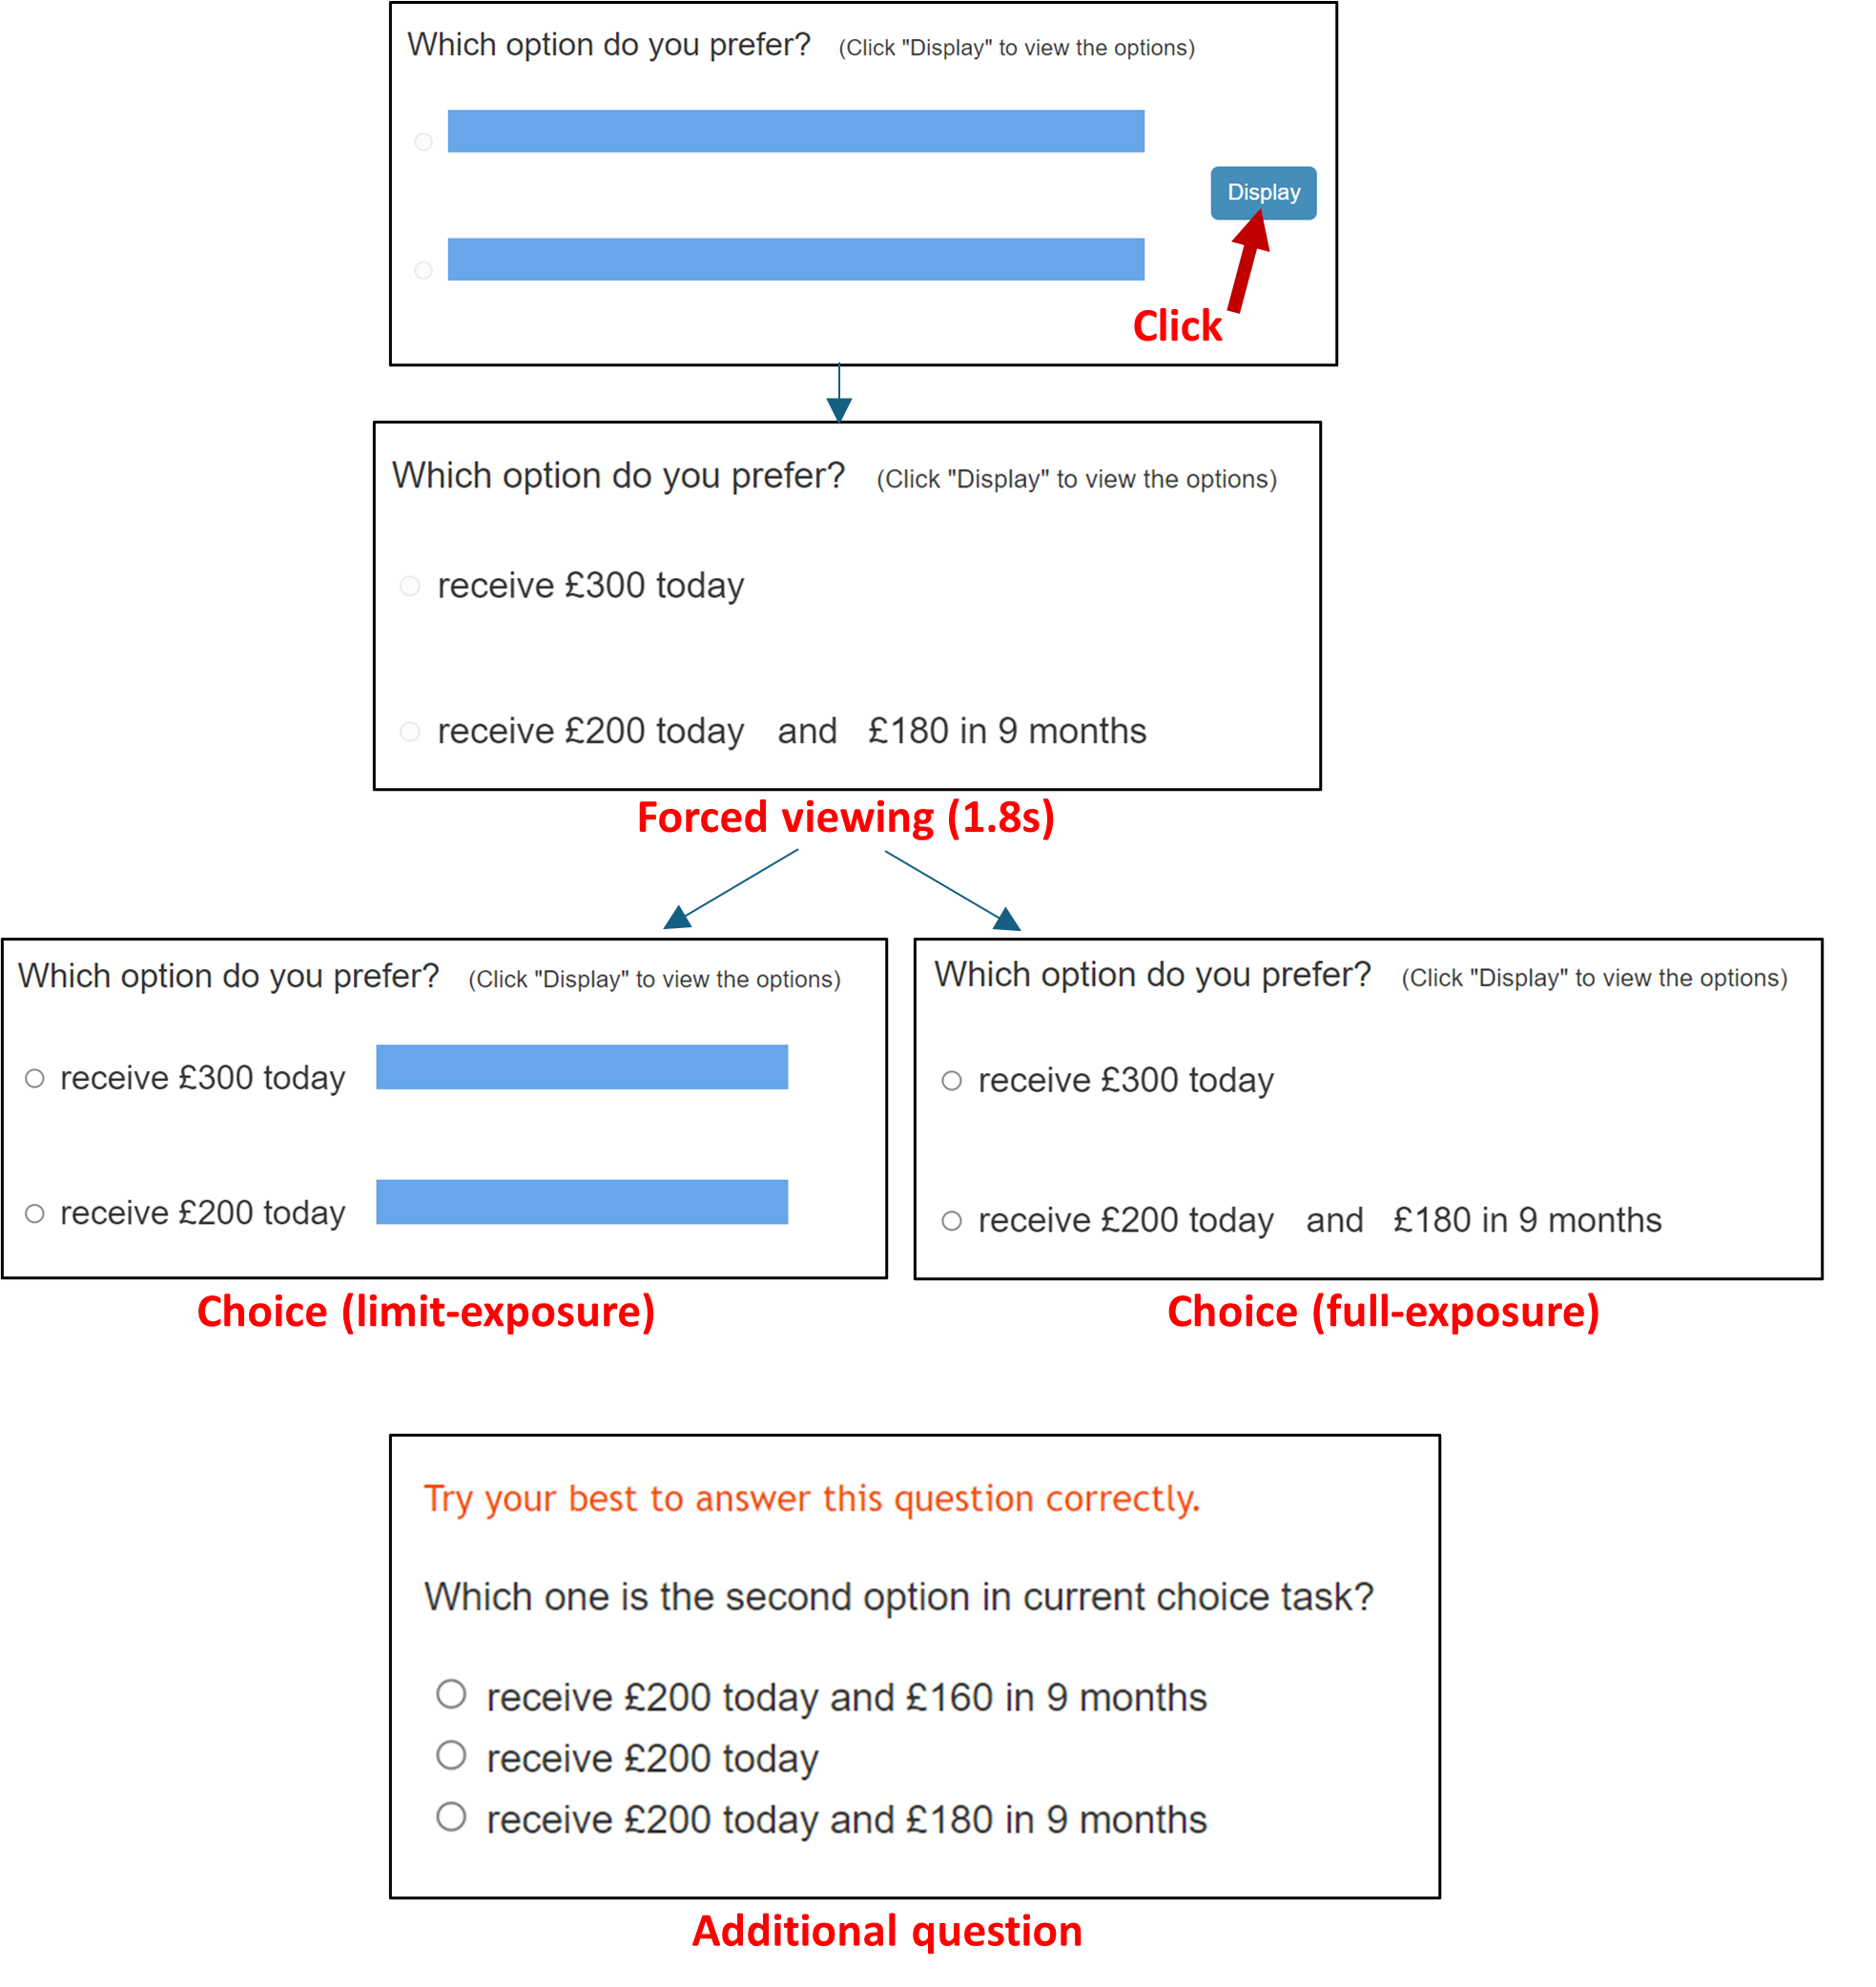
\includegraphics[width=\linewidth]{figures/exp3_intertemporal_task.png}
    \subcaption{Intertemporal Choice Task}
  \end{subfigure}
  \begin{subfigure}{\textwidth}
    \vspace{2.5em}
    \centering
    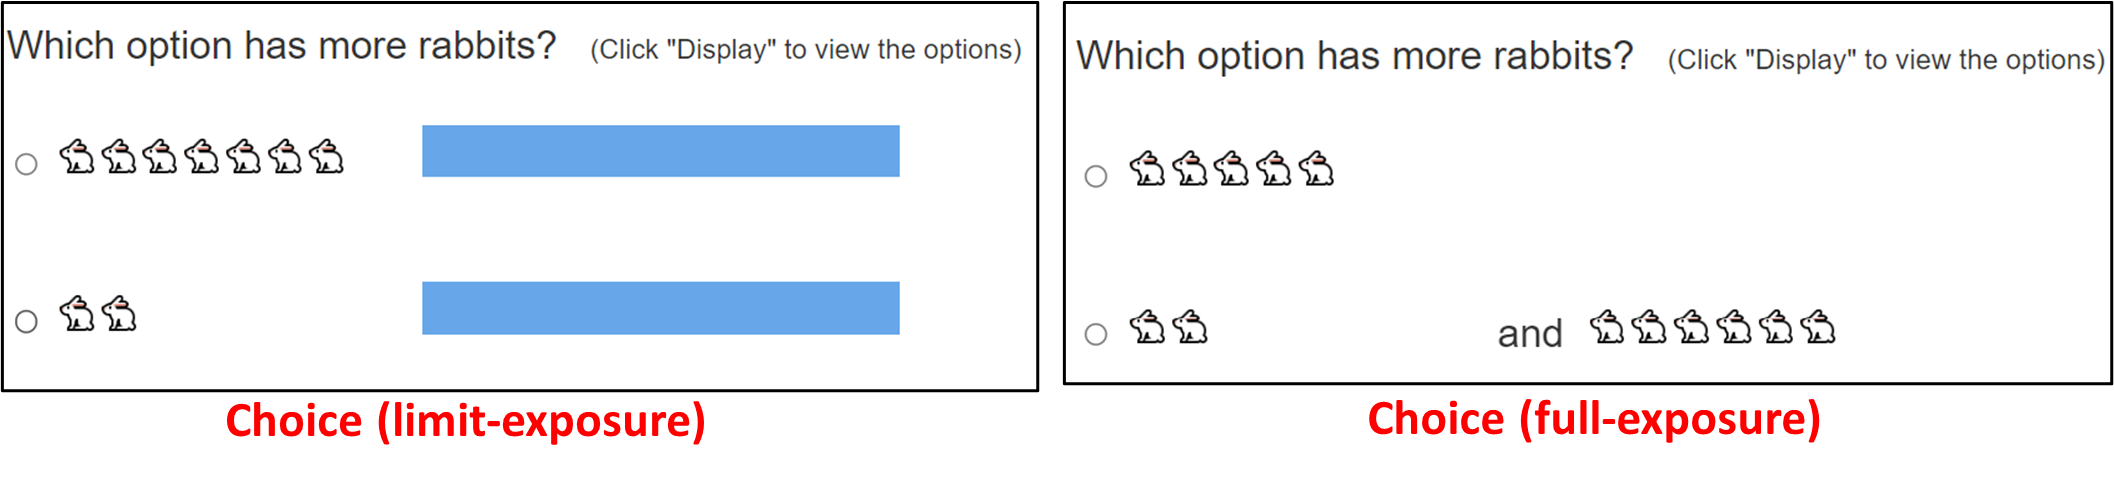
\includegraphics[width=\linewidth]{figures/exp3_rabbit_task.png}
    \subcaption{Count-the-Rabbits Task}
  \end{subfigure}
  \caption{Screenshot of Experiment 3}
  \label{fig:exp3_screenshot}
\end{figure}

In each intertemporal choice task, the single option could be denoted by
``receive \(s\) today'' and the sequence option by ``receive
\(\rho \eta\) today and \(1.5(1-\rho)\eta\) in 12 months''. In other
words, by choosing the single option, a decision maker would immediately
get an amount \((1-\rho)\eta\) more than the immediate reward in the
sequence option; by choosing the sequence option, the same amount
\((1-\rho)\eta\) would be invested in a riskless bond and the decision
maker would get an interest of 50\% in one year later. The preference
for the sequence option could be an indicator for patience. We select
\(\eta\) from \{£200, £240, £280, £320\} and \(\rho\) from \{0.1, 0.2,
0.3, 0.4, 0.5, 0.6\}. The largest level for \(\rho\) is 0.6, ensuring
that the delayed reward in the sequence option would be a considerable
amount (at least as the same as the immediate reward). Thus, the main
tasks in Part 1-2 contain 24 tasks. We randomly and evenly assign these
tasks to each part.

For each count-the-rabbit task, suppose the single option contains
\(r_1\) rabbits and the sequence option contains \(r_2\) rabbits for the
first bunch and \(r_3\) rabbits for the second bunch. We select \(r_1\)
from \{7, 8\}, \(r_2\) from \{1, 2, 3\}, and \(r_3\) from
\{\(r_1 - r_2 -1\), \(r_1 - r_2 +1\)\}. Therefore, there are 12 main
tasks in Part 3-4. In half of these tasks, the sequence option has one
more rabbit than the single option (\(r_2 + r_3 > r_1\)); for the other
half, it is the single option that has one more rabbit
(\(r_2 + r_3 < r_1\)). Similar to the intertemporal choice tasks, we
randomly and evenly assign these tasks to each part.

\hypertarget{sample}{%
\subsection{Sample}\label{sample}}

We recruited 300 UK residents via Prolific (female: 152; mean age:
43.6). The median completion time is 10.1 minutes. Each participant was
paid £1.5 (on average £8.1 per hour). In each of Part 1 and Part 2,
there is one attention check task. Four participants failed the
attention check. Besides, there were two participants for whom the tasks
were not displayed in the correct order.\footnote{For one participant,
  the data collected for main tasks in Part 2 ended up being example
  tasks. For the other participant, the data collected for the example
  count-the-rabbit tasks in Part 3 ended up being intertemporal choice
  tasks.} We drop the participants who fail the attention check and
those for whom the tasks were not displayed correctly. In the end, there
are 148 participants in the ``full-exposure'' group and 146 participants
in the ``limit-exposure'' group. We have 7,065 observations for
intertemporal choice tasks and 3,504 observations for count-the-rabbits
tasks.

The accuracy rate of additional questions is high for each kind of
tasks. For intertemporal choice tasks in Part 2, the overall accuracy
rate is 94.0\%, and 208 participants correctly answered all questions.
For count-the-rabbit tasks in Part 4, the overall accuracy rate is
96.7\%, and 259 participants correctly answered all questions.

\hypertarget{theoretical-analysis}{%
\subsection{Theoretical Analysis}\label{theoretical-analysis}}

In this experiment, we aim to investigate when people evaluate a
two-reward sequence, whether directing their attention to a considerable
delayed reward would make them value the sequence more. We divide
participants into two groups (limit-exposure / full-exposure). The
difference between these groups lies in the information they were
exposed to when making choices. Each participant experienced two parts
(no question / question). The setup of groups and questions was designed
to control participants' attention allocation during the tasks.

As is pointed out by \citet{chun2011taxonomy}, a critical function of
attention mechanisms is to ``focus limited processing capacity on the
most important information relevant to ongoing goals''. In the
``limit-exposure'' group, to achieve the goal of correctly answering the
additional questions, in each task participants have to remember the
(only) information being blocked out. Thus, in an intertemporal choice
task, they have to focus on the delayed reward in the sequence option
during the forced viewing period, as they can never access this
information after that. By contrast, in the ``full-exposure'' group, all
relevant information is visible when participants answer the additional
question, so they do not need to specifically focus on the delayed
reward. We propose, given the delayed reward is a considerable amount,
paying more attention to it would make participants value the sequence
option more. Therefore, for intertemporal choice tasks, being asked to
answer the additional question would increase the preference for the
sequence option for participants in the ``limit-exposure'' group, and
would not have much impact on the choices for participants in the
``full-exposure'' group.

The count-the-rabbits tasks can help us understand the mechanisms by
which attention influences choices. As is pointed out by
\citet{pleskac2023attention}, attention can alter choices by two
possible processes: one is through valuation, the other is directly
through perception. The latter suggests that attention increases the
perceived salience of an object and people may tend to choose the more
salient option. In specific preferential and perceptual decision tasks,
\citet{pleskac2023attention} find evidence supporting the valuation
process and contradicting the perceived salience process. Also, for our
experiment, we propose that attention alter intertemporal choices
through valuation rather than perception. The count-the-rabbit task (a
perceptual task) help us distinguish the two processes. These tasks
possess the same format as the intertemporal choice tasks, and as is
indicated by Figure \ref{fig:exp3_mean_choice}, under each group and
part, the frequency with which participants choose the sequence option
is similar between both kinds of tasks. If attention alters choice
mainly through perception for both tasks, the groups and additional
questions should influence the choices in the count-the-rabbits tasks in
the same way as in the intertemporal choice tasks. Indeed, the evidence
we found suggests they influence the choices in those tasks in different
ways, thus supports the valuation process.

Manipulating the exposure time of a stimuli is a commonly used technique
that can alter decision makers' attention and preferences in
experiments. For example, in one study of
\citet{fisher2021intertemporal}, participants are asked to choose
between a small sooner reward and a large later reward. The author
firstly presents the delay attribute and amount attribute in order. In
some choice tasks, the delay attribute is exposed for 2s while the
amount attribute is exposed for 0.5s. In other tasks, the exposure times
are reversed. The participants are then required to make a choice. The
author finds that when viewing the amount (delay) attribute,
participants tend to spend more time fixating at the large amount
(sooner date). When making the choices, they are more likely to choose
the large later reward if the amount attribute is exposed for a longer
time. Our experiment differ from \citet{fisher2021intertemporal} in two
ways. First, we direct attention to an element in a reward sequence,
rather than an attribute. Second, in our experiment, longer exposure
time does not necessarily mean more attention. As is suggested by Figure
\ref{fig:exp3_mouse_position}, for many participants, the intention to
choose an option has already been formed by the end of the forced
viewing period. That is, in the ``limit-exposure'' group, before we
block out some information, participants may have already made a
decision. Thus, we use the requirement to answer a relevant question to
raise attention to certain information rather than the exposure time
alone.

\hypertarget{choice-results}{%
\subsection{Choice Results}\label{choice-results}}

\hypertarget{intertemporal-choice-task}{%
\subsubsection{Intertemporal Choice
Task}\label{intertemporal-choice-task}}

The choices under each group and part, are distributed as in Figure
\ref{fig:exp3_mean_choice}. In the ``limit-exposure'' group, the
proportion of choosing the sequence option within the ``question'' part
is 5.5\% higher than that under the ``no question'' part; in the
``full-exposure'' group, the former proportion is 2.1\% higher than the
latter proportion. Besides, in the ``limit-exposure'' group, 23
participants always choose the single-amount option and 21 participants
always choose the sequence option. In the ``full-exposure'' group, 31
participants always choose the single-amount option and 35 participants
always choose the sequence option.

\begin{figure}
  \centering
  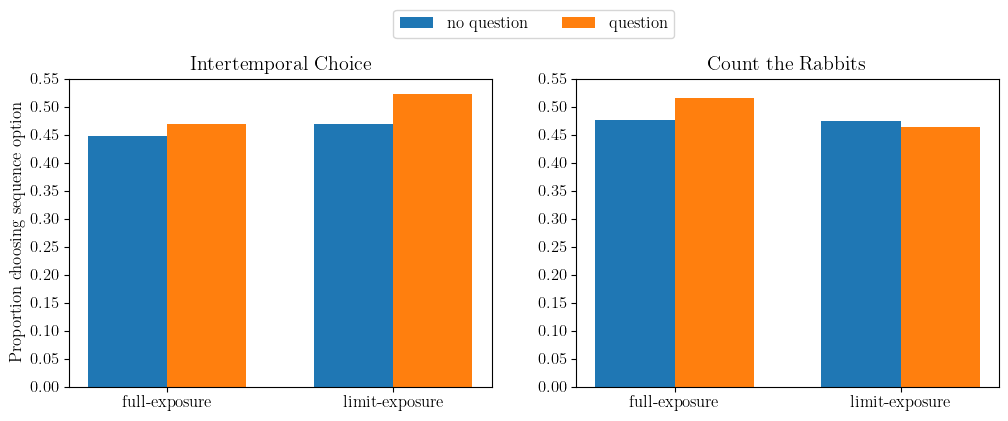
\includegraphics[width=\linewidth]{figures/seq_choice_ratio.png}
  \caption{Mean proportion of participants choosing the sequence option}
  \label{fig:exp3_mean_choice}
\end{figure}

We examine the impact of groups and questions on intertemporal choices
through a set of logistic linear regressions. Table
\ref{tab:exp3_reg_intertemporal_choice} illustrates the key estimates in
the results. The dependent variable is 1 if a participant choose the
sequence option in a task and 0 otherwise. The variable Group is 1 if
the participant is in the ``limit-exposure'' group and 0 otherwise;
Question is 1 if the task is within the ``question'' part and 0
otherwise. Each level of \(\rho\) and \(\eta\) is treated as a dummy
variable. Each of Model (1)-(3) in Table
\ref{tab:exp3_reg_intertemporal_choice} is estimated through maximum
likelihood method. Model (1) is a pooled regression. Model (2) is run
upon the sample in which each participant has changed her choice at
least once across all intertemporal choice tasks, and subject-specific
dummies are created for these participants.\footnote{The reason why
  Model (2) in Table \ref{tab:exp3_reg_intertemporal_choice} focuses on
  a subset of participants is, the design matrix will become singular
  without omitting those who keep choosing one option all the time.}
Model (3) is run upon the full sample and adds two dummies to Model (2)
to capture whether a subject always chooses the sequence option, and the
single option.


\documentclass[12pt]{article}


\begin{document}
\begin{table}
    \caption{Regression Results for Intertemporal Choice Tasks}
    \vspace*{12pt}
    \centering

      \begin{tabular}{llll}
\hline
 & (1) Pooled & (2) FE & (3) FE \\
\hline
Group & 0.082 & 0.034 & -0.1 \\
 & (0.189) & (0.102) & (0.096) \\
Question$\cdot1\{\text{Group}=0\}$ & 0.084 & 0.289 & 0.289 \\
 & (0.059) & (0.185) & (0.183) \\
Question$\cdot1\{\text{Group}=1\}$ & 0.223$^{***}$ & 0.535$^{***}$ & 0.535$^{***}$ \\
 & (0.067) & (0.162) & (0.161) \\
$1\{\rho=0.2\}$ & -0.276$^{***}$ & -0.756$^{***}$ & -0.756$^{***}$ \\
 & (0.051) & (0.135) & (0.133) \\
$1\{\rho=0.3\}$ & -0.333$^{***}$ & -0.915$^{***}$ & -0.915$^{***}$ \\
 & (0.059) & (0.156) & (0.155) \\
$1\{\rho=0.4\}$ & -0.254$^{***}$ & -0.688$^{***}$ & -0.688$^{***}$ \\
 & (0.061) & (0.166) & (0.164) \\
$1\{\rho=0.5\}$ & -0.193$^{**}$ & -0.516$^{**}$ & -0.516$^{**}$ \\
 & (0.071) & (0.194) & (0.192) \\
$1\{\rho=0.6\}$ & -0.468$^{***}$ & -1.281$^{***}$ & -1.281$^{***}$ \\
 & (0.081) & (0.22) & (0.218) \\
$1\{s=240\}$ & 0.191$^{***}$ & 0.53$^{***}$ & 0.53$^{***}$ \\
 & (0.044) & (0.119) & (0.118) \\
$1\{s=280\}$ & 0.665$^{***}$ & 1.795$^{***}$ & 1.795$^{***}$ \\
 & (0.058) & (0.126) & (0.125) \\
$1\{s=320\}$ & 0.475$^{***}$ & 1.293$^{***}$ & 1.293$^{***}$ \\
 & (0.053) & (0.124) & (0.123) \\\hline

observations & 7056 & 4416 & 7056 \\
aic & 9621.97 & 4294.947 & 4303.619 \\
\hline
\end{tabular}
% INSERT reg_choice

    \vspace*{4pt}
    \centering
    \begin{minipage}{0.85\textwidth}
    {\par\footnotesize Note: * $p<0.05$, ** $p<0.01$, *** $p<0.001$. Standard errors are clustered at the subject level and are reported in the parentheses. The p-values are calculated based on Wald tests. FE denotes fixed effects. Subject-specific dummies are omitted in this table.}
    \end{minipage}
    \label{tab:manipulate_intertemporal_choice}
\end{table}

\end{document}



As is consistent with our theoretical analysis, in the
``limit-exposure'' group (i.e.~Group = 1), participants are
significantly more likely to choose the sequence option within the
``question'' part rather than within the ``no question'' part (at
significance level 0.5\%). By contrast, in the ``full-exposure'' group
(i.e.~Group = 0), the additional questions do not increase the
preference for the sequence option significantly. In addition, with
\(\eta\) growing larger, participants are more likely to choose the
sequence option, which is in line with the magnitude effect.

\hypertarget{count-the-rabbits-task}{%
\subsubsection{Count-the-Rabbits Task}\label{count-the-rabbits-task}}

In count-the-rabbits tasks, 226 participants correctly choose the option
with more rabbits for every task, and the overall accuracy rate is
97.0\%. There are only 105 wrong choices. As is illustrated in Figure
\ref{fig:exp3_wrong_rabbits}, the wrong choices in count-the-rabbits
tasks are disproportionally biased to the single option. In all
conditions except the ``question'' part in the ``full-exposure'' group,
participants are more likely to choose the single option by mistake,
rather than the sequence option. One explanation is that, in the
``full-exposure'' group, to answer the additional questions,
participants need to (and they can) count the rabbits within each bunch,
which helps eliminating the choice error.

\begin{figure}
  \centering
  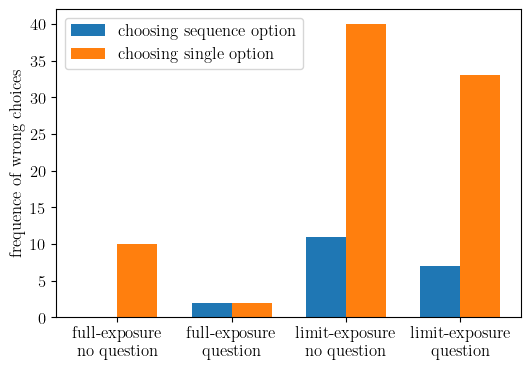
\includegraphics[width=0.75\linewidth]{figures/wrong_rabbit_choice.png}
  \caption{Frequence of wrong choices in count-the-rabbits tasks}
  \label{fig:exp3_wrong_rabbits}
\end{figure}

Furthermore, we conduct a set of logistic linear regressions upon the
choices in the count-the-rabbits tasks. Table
\ref{tab:exp3_reg_rabbit_choice} illustrates the key estimates. The
dependent variable, and variable Group as well as Question are the same
as those for the intertemporal choice tasks. Each level of \(r_1\) and
\(r_2\) is treated as a dummy variable. We also created a dummy variable
for whether the sequence option has more rabbits (i.e.
\(r_2 + r_3 > r_1\)). Model (1)-(4) in Table
\ref{tab:exp3_reg_rabbit_choice} are all estimated through maximum
likelihood method. Model (1) is a pooled regression while Model (2)-(4)
include subject-specific dummies. Model (2) are run upon the full
sample, Model (3) is run upon the sample in which each participant has
changed her choice at least once across all intertemporal choice tasks,
Model (4) is run upon the sample in which each participant has made at
least one wrong choice in count-the-rabbits tasks. Notably, in the
``limit-exposure'' group, participants are significantly more likely to
choose the sequence option within the ``question'' part, whereas in the
``full-exposure'' group, the additional questions have no significant
impact on choices. In other words, compared with the intertemporal
choice tasks, adding the additional questions to the count-the-rabbits
tasks produces a reverse effect on choice for participants in each
group. This result provides a supportive evidence for our argument that
attention increases the preference for the sequence option in our
intertemporal choice tasks through valuation rather than perception.


\documentclass[12pt]{article}


\begin{document}
\begin{table}
    \caption{Regression Results for Count-the-Rabbits Tasks}
    \vspace*{12pt}
    \centering

      \begin{tabular}{lllll}
\hline
 & (1) Pooled & (2) FE & (3) FE & (4) FE \\
\hline
Group & -0.73$^{*}$ & -4.379$^{***}$ & -0.158 & -0.757 \\
 & (0.33) & (1.114) & (8.618) & (0.392) \\
Question$\cdot1\{\text{Group}=0\}$ & 0.574$^{*}$ & 1.378$^{*}$ & 1.56$^{*}$ & 2.005$^{**}$ \\
 & (0.226) & (0.6) & (0.689) & (0.744) \\
Questsion$\cdot1\{\text{Group}=1\}$ & 0.062 & 0.152 & 0.391 & 0.145 \\
 & (0.318) & (0.368) & (0.422) & (0.344) \\
$1\{r_2 + r_3 > r_1\}$ & 7.797$^{***}$ & 11.71$^{***}$ & 11.198$^{***}$ & 6.181$^{***}$ \\
 & (0.377) & (1.091) & (1.249) & (0.552) \\
$1\{r_2 =2\}$ & 0.106 & 0.183 & 0.161 & 0.217 \\
 & (0.274) & (0.378) & (0.45) & (0.393) \\
$1\{r_2=3\}$ & -0.655$^{***}$ & -0.95$^{**}$ & -1.014$^{*}$ & -0.991$^{***}$ \\
 & (0.228) & (0.338) & (0.395) & (0.35) \\
$1\{r_1=8\}$ & 0.145 & 0.192 & 0.145 & 0.191 \\
 & (0.166) & (0.241) & (0.272) & (0.252) \\\hline

observations & 3504 & 3504 & 2190 & 810 \\
aic & 878.752 & 1100.636 & 746.754 & 583.857 \\
\hline
\end{tabular}
% INSERT reg_rabbit

    \vspace*{4pt}
    \centering
    \begin{minipage}{0.85\textwidth}
    {\par\footnotesize Note: * $p<0.05$, ** $p<0.01$, *** $p<0.005$. Standard errors are clustered at the subject level and are reported in the parentheses. The p-values are calculated based on Wald tests. FE denotes individual fixed-effects. Model (1)-(2) are run upon the full sample, (3) is for those having changed choices at least once in intertemporal choice tasks, (4) is for those having made wrong choices in count-the-rabbits tasks. Intercepts and subject-specific dummies are omitted in this table.}
    \end{minipage}
    \label{tab:exp3_reg_rabbit_choice}
\end{table}

\end{document}



\hypertarget{decision-process}{%
\subsection{Decision Process}\label{decision-process}}

To examine the participants' decision processes, we record the
participants' mouse position at the moment when they are prompted to
make a choice (i.e.~the end of the forced viewing period), and their
response time in each choice task.

First, the mouse position data suggests, for many participants, the
intention to choose an option may have already been formed at the end of
the forced viewing period. As is illustrated by Figure
\ref{fig:exp3_screenshot}, the single option lies above the sequence
option in each choice task. When a participant click the ``Display''
button to view the content of options, her mouse pointer should lie in
the middle between the two options. After that, she can move the mouse
freely though the mouse pointer is invisible. Then, when the pointer
appears again, she is asked to make a choice. Figure
\ref{fig:exp3_mouse_position} shows, at the moment when participants are
asked to make a choice, for those who eventually choose the sequence
(single) option, the peak of the distribution of their mouses' vertical
positions is exactly at the position of the option they want to choose.
This indicates that, at that moment, such participants have already had
a decision in mind and moved their mouses toward the option they tend to
choose. For such participants, if our experimental conditions has a
causal effect on their choices, it should occur in the forced viewing
period.

\begin{figure}
  \centering
  \begin{subfigure}{\textwidth}
    \centering
    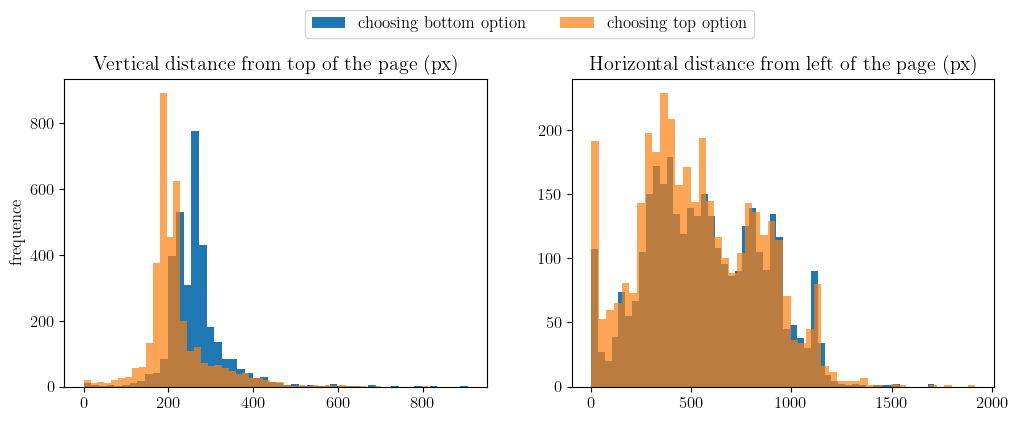
\includegraphics[width=\linewidth]{figures/mouse_intertemporal.png}
    \subcaption{Intertemporal Choice Task}
  \end{subfigure}
  \begin{subfigure}{\textwidth}
    \vspace{1.5em}
    \centering
    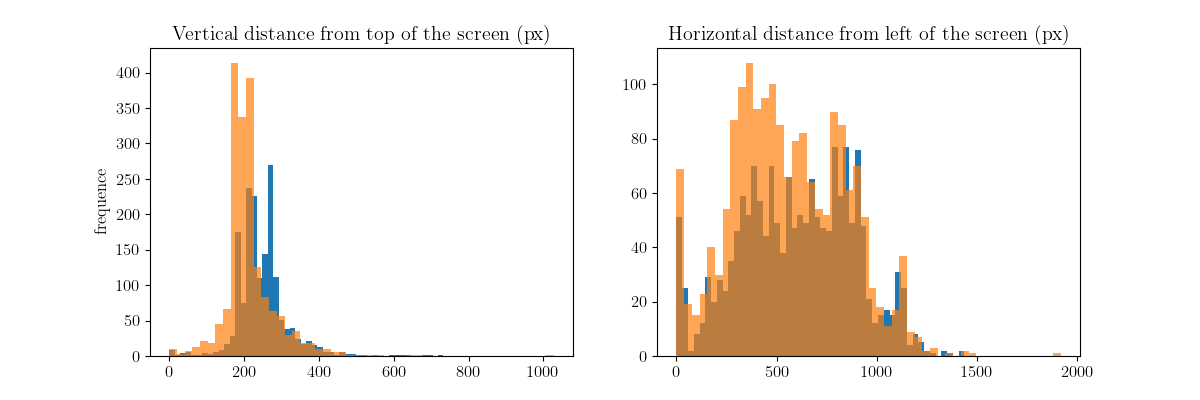
\includegraphics[width=\linewidth]{figures/mouse_rabbit.png}
    \subcaption{Count-the-Rabbits Task}
  \end{subfigure}
  \caption{Mouse positions recorded at the end of the forced viewing period}
  \label{fig:exp3_mouse_position}
\end{figure}

Second, for response time, we conducted linear regressions with 2SLS
method. We use data collected from those who have changed choices at
least once across the intertemporal choices tasks as the sample. For
first-stage regressions, we use Model (2) in Table
\ref{tab:exp3_reg_intertemporal_choice} to predict choices in
intertmporal choice tasks, and use Model (3) in Table
\ref{tab:exp3_reg_rabbit_choice} to predict choices in count-the-rabbits
tasks. We construct a variable Choice which is 1 if the predicted choice
is the sequence option and is 0 otherwise. For second-stage regressions,
the dependent variable is the response time (in second). We use the
variables in Table \ref{tab:exp3_reg_intertemporal_choice} and Table
\ref{tab:exp3_reg_rabbit_choice}, their interactions with Choice, and
subject-specific dummies as the independent variables. Given the
response time data contain some outliers, we exclude the highest 0.5\%
response times. The key estimates are reported in Table
\ref{tab:exp3_reg_response_time}.

Notably, in Table \ref{tab:exp3_reg_response_time}, the coefficients for
the interaction between Choice and Group are significantly negative.
This indicates that the ``limit-exposure'' group facilitates the choice
toward the sequence option in comparison of the ``full-exposure'' group.
However, as is illustrated by Table
\ref{tab:exp3_reg_intertemporal_choice} and Table
\ref{tab:exp3_reg_rabbit_choice}, Group has no impact on the choice
outcome in intertemporal choice tasks. These results provides insights
on how attention may affect valuation in intertemporal choices. Being
informed that there is some information to be blocked makes the sequence
option capture participants' attention. However, this has no impact on
valuation. Only when participants intentionally pay attention to learn
the (semantic) information about the rewards, can the option value be
increased.


\begin{table}[!h]
    \caption{Predicting response times with choices and conditions in Experiment 1}
    \vspace*{10pt}
    \centering

      \begin{tabular}{lll}
\hline
 & Intertemporal Choice & Count-the-Rabbits \\
\hline
Group & -0.684$^{***}$ & -0.792$^{***}$ \\
 & (0.141) & (0.144) \\
Question$\cdot1\{\text{Group}=0\}$ & -0.165 & 0.912$^{***}$ \\
 & (0.174) & (0.199) \\
Question$\cdot1\{\text{Group}=1\}$ & 0.457$^{***}$ & 0.849$^{***}$ \\
 & (0.101) & (0.132) \\
Choice & 0.954$^{*}$ & 1.291$^{***}$ \\
 & (0.399) & (0.456) \\
Choice$\times$Group & -0.762$^{*}$ & -1.265$^{***}$ \\
 & (0.304) & (0.229) \\
Choice$\times$Question$\cdot1\{\text{Group}=0\}$ & 0.001 & -0.138 \\
 & (0.257) & (0.23) \\
Choice$\times$Question$\cdot1\{\text{Group}=1\}$ & -0.12 & 0.263 \\
 & (0.195) & (0.175) \\\hline

observations & 4393 & 2179 \\
AIC & 18560.034 & 8711.872 \\
adj-$R^2$ & 0.381 & 0.55 \\
\hline
\end{tabular}
% INSERT reg_response_time

    \vspace*{4pt}
    \centering
    \begin{minipage}{0.85\textwidth}
    {\par\footnotesize Note: * $p<0.05$, ** $p<0.01$, *** $p<0.005$. Both models are estimated through 2SLS method. For first-stage regression, we use the model for Column (2) in Table \ref{tab:exp3_reg_intertemporal_choice} to predict intertemporal choices, and the model for Column (3) in Table \ref{tab:exp3_reg_rabbit_choice} to predict count-the-rabbits choices. The variable Choice which is 1 if the predicted choice is the sequence option and is 0 otherwise. For second-stage regression, indepdent variables are the predictors shown in the table plus task-specific dummies and their interactions with Choice, and participant-specific dummies. Standard errors (in the parentheses) are clustered at the subject level. $p$-values are calculated based on t-tests. }
    \end{minipage}
    \label{tab:exp3_reg_response_time}
\end{table}




\renewcommand\refname{Reference}
  \bibliography{experiment-3-ref.bib}

\end{document}
